%!TEX root = ../../presentation.tex

\begin{frame}[plain]{Monitoring Program Flow Trace: Tools}
  \textwidthplain
  \centering
  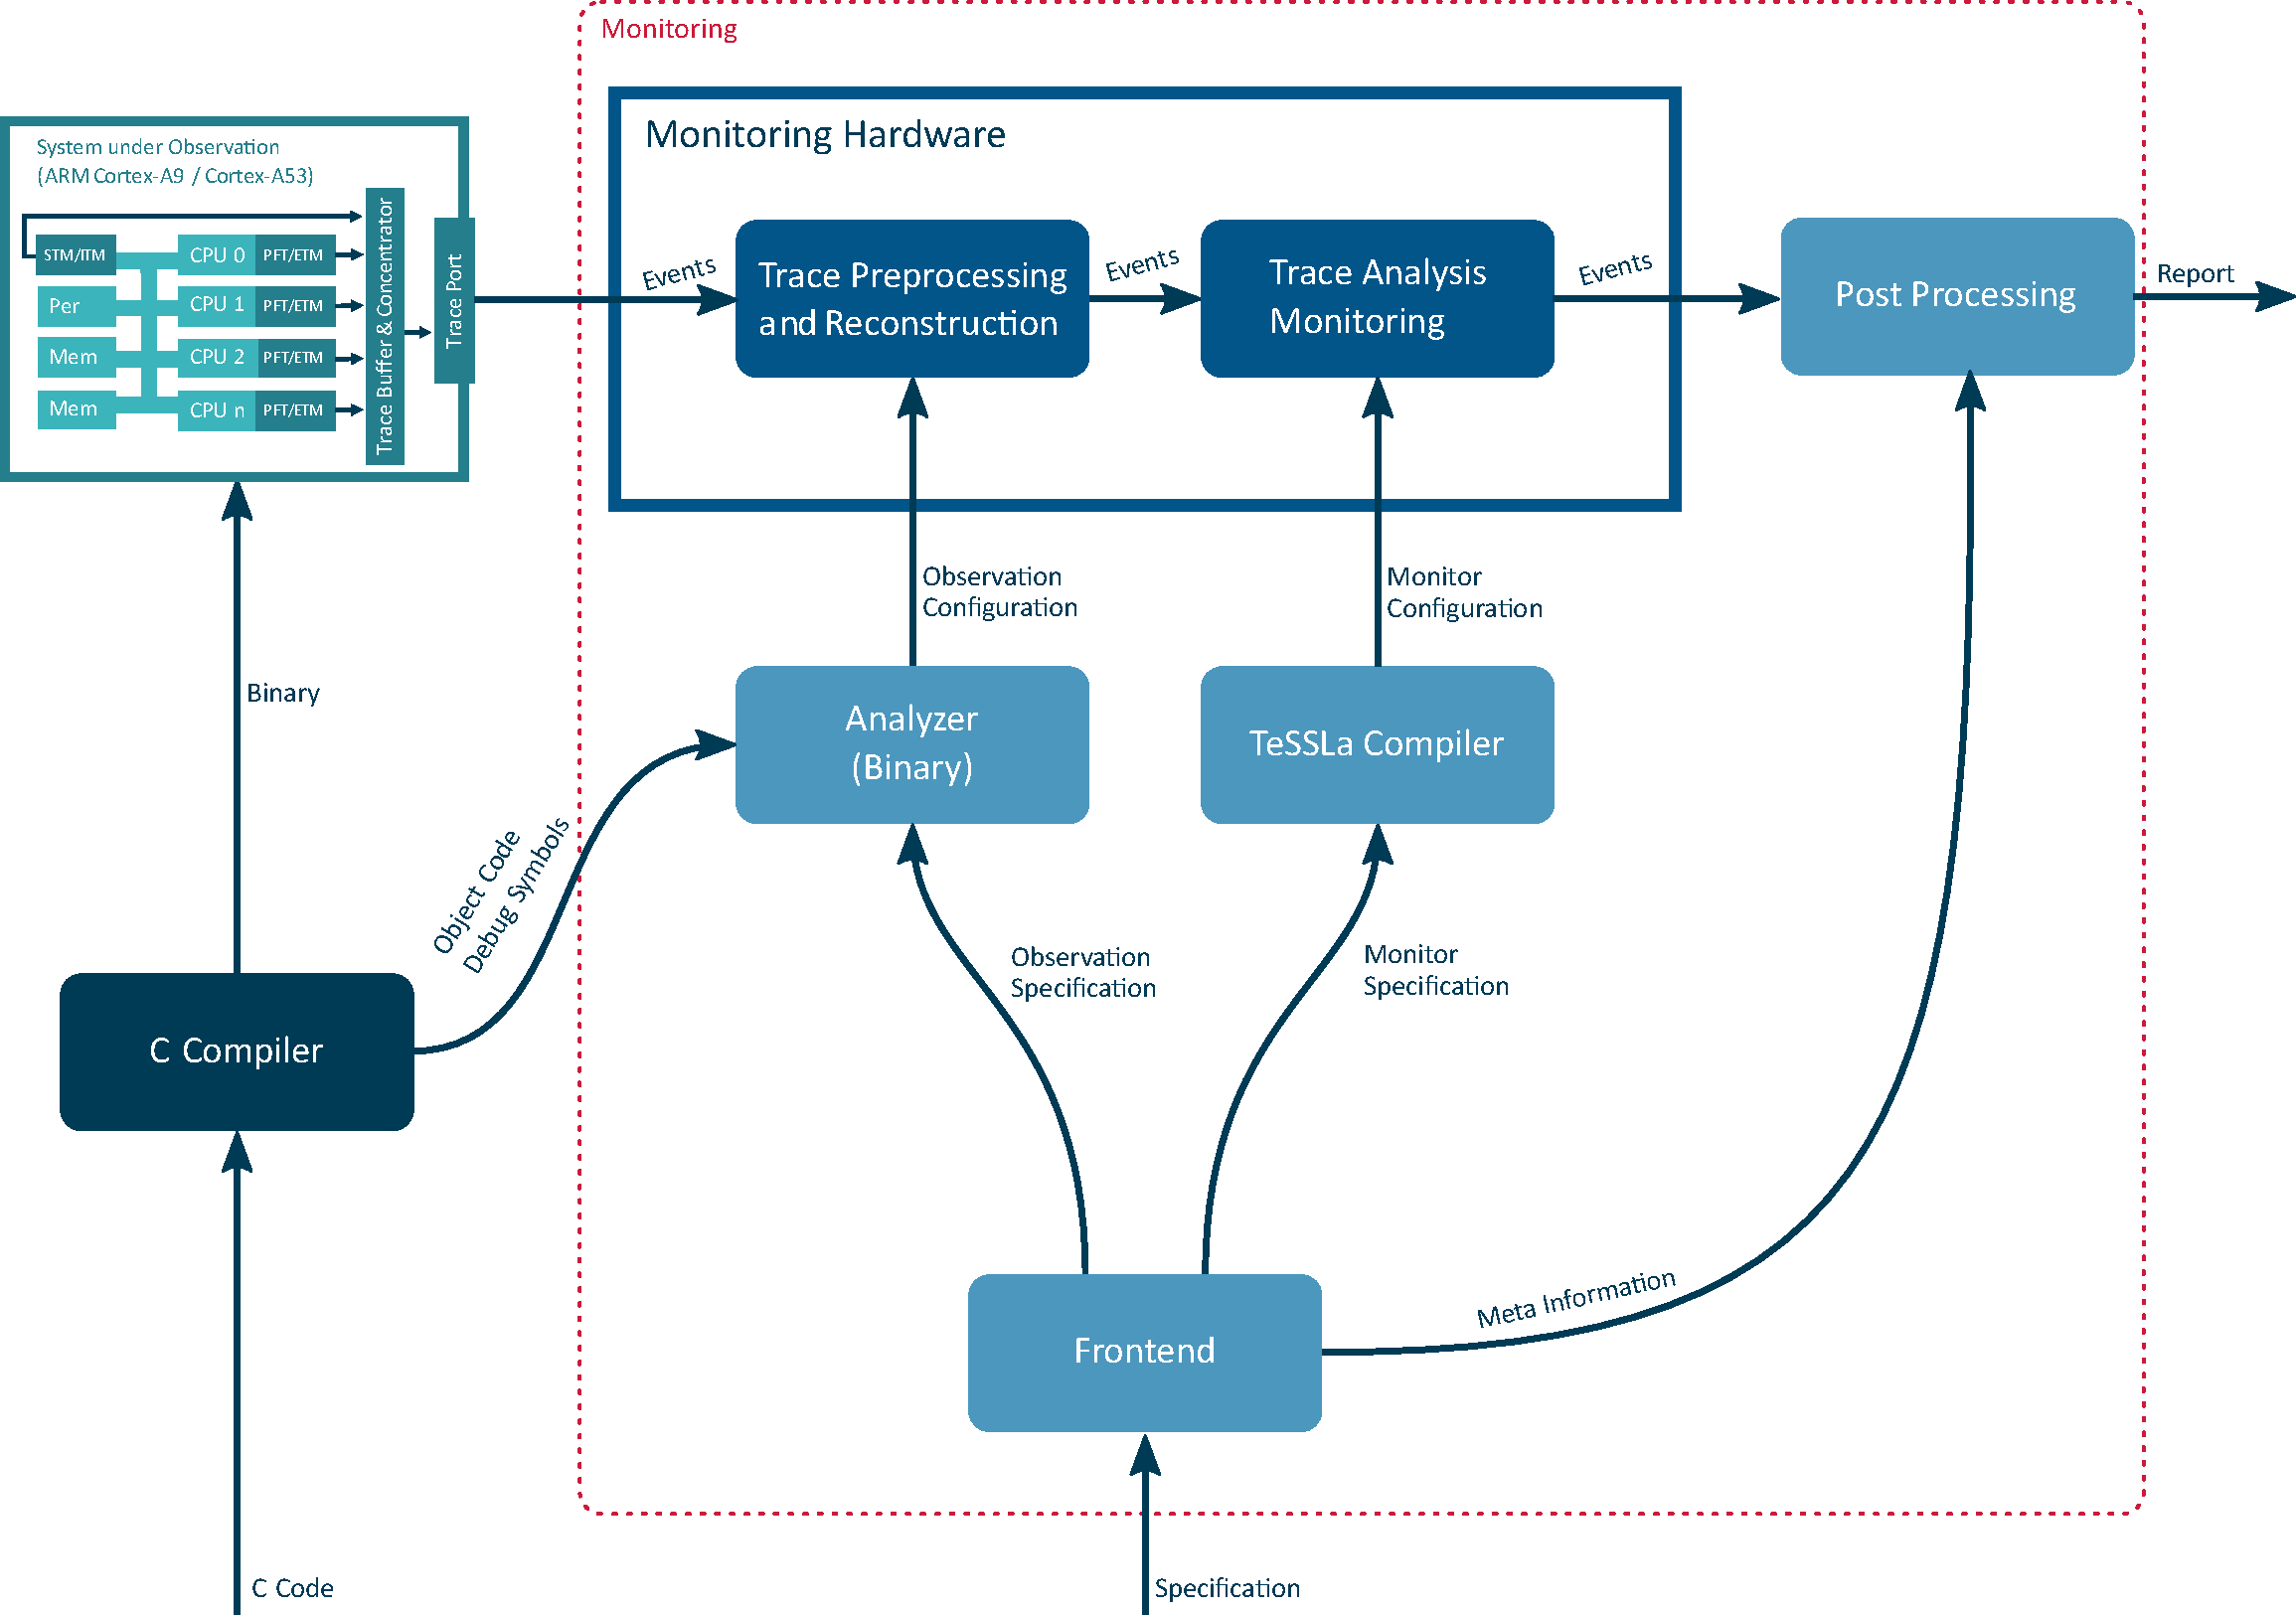
\includegraphics[width=.9\textwidth]{content/chapter_hardware_srv/overview-program-trace.pdf}
\end{frame}

\begin{frame}[t,plain,fragile]{Trace Reconstruction}
  \textwidthplain
  \vskip-4ex
  \hfill
  \tikzset{
    L1/.style={},
    L1a/.style={},
    L1b/.style={},
    L2/.style={},
    L3/.style={},
    L1no/.style={},
    L1yes/.style={},
    L1ano/.style={},
    L1ayes/.style={},
    L1byes/.style={},
    L2yes/.style={},
    active node/.style={draw=alertedcolor,fill=alertedcolor!18},
    active edge/.style={alertedcolor}
  }
  \newcommand{\highlight}[2]{\uncover<#1->{\alt<#1>{\colorbox{alertedcolor!18}{\strut #2}}{\colorbox{white}{\strut #2}}}}
  \newcommand{\highlightEmpty}[1]{\uncover<#1->{\colorbox{white}{\strut}}}
  \only<2>{\tikzstyle{L1}=[active node]}
  \only<3>{\tikzstyle{L1a}=[active node]\tikzstyle{L1no}=[active edge]}
  \only<4>{\tikzstyle{L1b}=[active node]\tikzstyle{L1ano}=[active edge]}
  \only<5>{\tikzstyle{L1}=[active node]\tikzstyle{L1byes}=[active edge]}
  \only<6>{\tikzstyle{L1a}=[active node]\tikzstyle{L1no}=[active edge]}
  \only<7>{\tikzstyle{L2}=[active node]\tikzstyle{L1ayes}=[active edge]}
  \only<8>{\tikzstyle{L1}=[active node]\tikzstyle{L2yes}=[active edge]}
  \only<9>{\tikzstyle{L3}=[active node]\tikzstyle{L1yes}=[active edge]}
  \begin{tikzpicture}[
      every node/.style={inner sep=1pt, font=\small},
      every state/.append style={inner sep=0pt, minimum size=22pt},
      shorten >=1pt,
      auto, thick, node distance=-1mm and 15mm
    ]
    \node[state, initial, L1] (L1) {L1};
    \node[state, right=8mm of L1, L1a] (L1a) {L1a};
    \node[state, above right=of L1a, L1b] (L1b) {L1b};
    \node[state, below right=of L1a, L2] (L2) {L2};
    \node[state, below=5mm of L1, L3] (L3) {L3};

    \path[->]
      (L1) edge[L1yes] node[swap] {yes} (L3)
      (L1) edge[L1no] node {no} (L1a)
      (L1a) edge[L1ayes, bend right=10] node[near end, swap] {yes/odd} (L2)
      (L1a) edge[L1ano, bend left=10] node[near end] {no/even} (L1b)
      (L1b) edge[L1byes, bend right=60, looseness=.5] node[swap, near start] {yes} (L1)
      (L2) edge[L2yes, bend left=60, looseness=.5] node[near start] {yes} (L1);
  \end{tikzpicture}

  \lstset{basicstyle=\ttfamily\scriptsize}

  \begin{columns}[t]
    \column{3.3cm}
    \inhead{C Code}
    \vskip-2pt
    \begin{lstlisting}[
        gobble=6,
        language=C,
        linebackgroundcolor={%
          \btLstHL<1>{}%
          \btLstHL<2>{2}%
          \btLstHL<3>{5}%
          \btLstHL<4>{9-10}%
          \btLstHL<5>{2}%
          \btLstHL<6>{5}%
          \btLstHL<7>{12-13}%
          \btLstHL<8>{2}%
          \btLstHL<9>{}%
        }]

      while (n > 1) {


        if (n % 2 == 0) {



          // even
          n = n / 2;
        } else {
          // odd
          n = 3 * n + 1;
        }
      }
    \end{lstlisting}

    \column{3.3cm}
    \inhead{Assembler}
    \vskip-2pt
    \begin{lstlisting}[
        gobble=6,
        language={},
        morekeywords={cmp,ble,bne,b},
        morekeywords={[2]L1,L1a,L1b,L2,L3},
        linebackgroundcolor={%
          \btLstHL<1>{}%
          \btLstHL<2>{2-3}%
          \btLstHL<3>{5-7}%
          \btLstHL<4>{9-10}%
          \btLstHL<5>{2-3}%
          \btLstHL<6>{5-7}%
          \btLstHL<7>{12-14}%
          \btLstHL<8>{2-3}%
          \btLstHL<9>{}%
        }]
      .L1:
            cmp $n, 1
            ble .L3
      .L1a:
            $tmp = $n % 2
            cmp $tmp, 0
            bne .L2
      .L1b:
            $n = $n / 2
            b .L1
      .L2:
            $n = 3 * $n
            $n = $n + 1
            b .L1
      .L3:
    \end{lstlisting}

    \column{1cm}
    \inhead{Branch\\taken?\\[1ex]}

    \highlight{3}{no}\\[-1ex]
    \highlight{4}{no}\\[-1ex]
    \highlight{5}{yes}\\[-1ex]
    \highlight{6}{no}\\[-1ex]
    \highlight{7}{yes}\\[-1ex]
    \highlight{8}{yes}\\[-1ex]
    \highlight{9}{yes}

    \column{1cm}
    \inhead{Events\\~\\[1ex]}

    \highlightEmpty{3}\\[-1ex]
    \highlight{4}{even}\\[-1ex]
    \highlightEmpty{5}\\[-1ex]
    \highlightEmpty{6}\\[-1ex]
    \highlight{7}{odd}
  \end{columns}
\end{frame}

\begin{frame}{Multithreading}
  \inhead{Problem: Distinguish multiple threads}
  \begin{itemize}
    \item We can only \alert{distinguish instructions} traced from\\ \alert{different cores}.
    \item Scheduler can execute \alert{multiple threads\\ on the same core}.
    \item Context switch reconfigures MMU\\
      \alert{$\Longrightarrow$ Same logical addresses used in different threads.}
  \end{itemize}

  \vskip3ex

  \inhead{Solution: Context ID Register}
  \begin{enumerate}
    \item OS writes \alert{thread ID} to \alert{context ID register}.
    \item Tracing unit generates \alert{context ID message}.
    \item Trace reconstruction \alert{changes lookup table}\\
      for the program flow reconstruction information.
  \end{enumerate}
\end{frame}
